\documentclass[11pt]{article}
\usepackage[T1]{fontenc}
\usepackage{lmodern}
\usepackage[margin=2.4cm]{geometry}
\usepackage{amsmath,amssymb}
\usepackage{booktabs}
\usepackage{graphicx}
\usepackage{array}
\usepackage{caption}
\usepackage[numbers,sort&compress]{natbib}
\usepackage[hidelinks]{hyperref}
\usepackage{xcolor}
\captionsetup{font=small,labelfont=bf}
\setlength{\tabcolsep}{4.5pt}

\title{Predicting Where People Look at Ads:\\An Open Benchmark and a Compact Attention Model\\Fine-Tuned on Design Eye Tracking}
\author{Pratyush Mahapatra\\[2pt]
\small Independent researcher \quad \url{https://pranikz.dev}\\[2pt]
\small Code, model and data pointers: \url{https://github.com/pranikz/MediaAttention}}
\date{October 2026}

\begin{document}
\maketitle

\begin{abstract}
Predicted-attention tools are widely used to pre-test advertising, yet their accuracy claims are hard to compare and
the best open models were trained on natural photographs rather than designed content. We make three contributions.
First, we review 15 commercial predictive-attention tools from public sources and show that headline claims of
``92--95\% accuracy'' are mostly AUC expressed as a share of the inter-observer ceiling, a saturated metric on which a
centre-only prior already scores 0.78 on MIT300. Second, we benchmark six openly available models, from a 3.7M-parameter
network to the 452M-parameter DeepGaze MSDB, against human eye tracking on webpages (FiWI) and on 1,980 posters, app
screens and webpages (UEyes), none of which they were trained on. On design content, model size does not buy accuracy:
DeepGaze MSDB reaches a correlation (CC) of 0.485 with human fixation maps on UEyes, tied with DeepGaze IIE and below
the 3.7M-parameter UNISAL (0.502). Third, we fine-tune UNISAL on the UEyes training split. The resulting model,
MediaAttention-Ads v1, reaches CC 0.735 on the held-out UEyes test split and 0.752 on held-out posters, against 0.514
and 0.496 for the best other open model, with non-overlapping 95\% confidence intervals, while also improving on
out-of-domain webpages (0.631 vs.\ 0.616). The model runs in 0.04\,s per image on a laptop. We release the model under
Apache-2.0 together with MediaAttention, an open toolkit that turns attention maps into advertising metrics, and an
open browser-based eye-tracking study kit.
\end{abstract}

\section{Introduction}
Attention is the first gate in advertising: an element that is not looked at cannot persuade or be remembered.
Eye-tracking studies of print advertising show that pictures, text size and brand placement shape where attention goes
and how it transfers between elements~\cite{pieters2004attention,pieters2010stopping}, and visual salience alone can bias
quick consumer choices~\cite{milosavljevic2012saliency}. Measuring attention with eye tracking is accurate but slow and
costly, so a market has grown around \emph{predicting} it: a creative is uploaded and a heatmap and scores come back.

Two problems limit this practice. Commercial tools quote accuracy on different metrics, test sets and viewing durations,
often on their own data, so their claims cannot be compared. And the open models that lead public benchmarks were
trained mostly on natural photographs (SALICON~\cite{jiang2015salicon}, MIT1003~\cite{judd2009learning}), while
advertising is dense with type, logos and layout. This paper contributes:
\begin{enumerate}
\item A review of 15 commercial predictive-attention tools that decodes what their accuracy claims measure (Section~\ref{sec:commercial}).
\item An open benchmark of six models against human eye tracking on webpages, posters and user interfaces none of them
were trained on, including a full run of the 452M-parameter DeepGaze MSDB (Section~\ref{sec:results}).
\item MediaAttention-Ads v1, a 3.7M-parameter attention model fine-tuned on design eye tracking that leads every open
model on posters, ads and interfaces by a wide margin (Sections~\ref{sec:method} and~\ref{sec:results}).
\item MediaAttention, an open-source toolkit that turns attention maps into advertising metrics, and an open browser
study kit for collecting eye-tracking and implicit-response data (Section~\ref{sec:method}).
\end{enumerate}

\section{Background and related work}
\paragraph{Attention prediction.} Computational saliency began with feature-contrast models~\cite{itti1998model}. Since
2015, deep networks trained on large fixation datasets dominate. DeepGaze IIE~\cite{linardos2021deepgaze} ensembles
four ImageNet backbones; DeepGaze MSDB~\cite{kummerer2025msdb} combines CLIP and DINOv2 features at several scales with
dataset-bias parameters; TranSalNet~\cite{lou2022transalnet} adds a transformer encoder to a DenseNet; UNISAL~\cite{droste2020unisal}
is a compact network for both images and video. The MIT/T\"ubingen benchmark~\cite{kummerer2018benchmarking,mit300}
evaluates models on held-out data and is the closest the field has to a neutral scoreboard.

\paragraph{Design and interface saliency.} Design-oriented eye-tracking data is rare. FiWI~\cite{shen2014webpage}
covers 149 webpages; UEyes~\cite{jiang2023ueyes} covers 1,980 posters, webpages, desktop and mobile interfaces viewed
by 62 participants. SUM~\cite{hosseini2024sum} trains on several datasets including UEyes. For video advertising,
recent work finds video models far ahead of frame-by-frame image models on TV ads~\cite{ye2026viasnet}.

\paragraph{Metrics.} No single metric captures prediction quality~\cite{bylinskii2019metrics}. AUC measures ranking and
saturates; shuffled AUC (sAUC) cancels centre bias~\cite{tatler2007central}; NSS, CC, SIM and KL divergence compare
maps. We use CC, the Pearson correlation between predicted and blurred human fixation maps, as the headline metric and
report the rest.

\section{What commercial accuracy claims measure}\label{sec:commercial}
We surveyed vendor websites, documentation and white papers in October 2026. Where a claim can be decoded, it is usually
AUC divided by the inter-observer ceiling: one vendor's ``92.5\%'' is its MIT300 AUC (0.864) divided by the gold
standard (0.934). On MIT300 every listed model scores between 0.84 and 0.89 AUC and a centre-only prior already reaches
0.78, so this ratio makes small differences look large. On CC the same tools separate clearly
(Table~\ref{tab:mit300}). Only four commercial tools have third-party-computed MIT300 entries, and all rank below the
best open models. The most detailed public technical document we found reports CC 0.944 on held-out data from the
vendor's own ad corpus~\cite{neurons2025tech}; it cannot be compared with MIT300 scores, which use a different test
set, ceiling and viewing duration. We found no external validation of secondary scores (clarity, memory, emotion).

\begin{table}[t]
\centering\small
\begin{tabular}{lrrrrrl}
\toprule
Model (MIT300) & AUC & sAUC & NSS & CC & KLD & Type \\
\midrule
DeepGaze MSDB & 0.894 & 0.816 & 2.74 & 0.883 & 0.254 & open, research \\
DeepGaze IIE & 0.883 & 0.794 & 2.53 & 0.824 & 0.347 & open, research \\
TranSalNet-Dense & 0.873 & 0.747 & 2.41 & 0.807 & 1.014 & open (MIT) \\
UNISAL & 0.877 & 0.784 & 2.37 & 0.785 & 0.415 & open (Apache-2.0) \\
Attention Insight & 0.864 & 0.745 & 2.18 & 0.758 & 0.887 & commercial \\
Emotiva & 0.864 & 0.770 & 2.20 & 0.743 & 0.496 & commercial \\
MedullEyes-V1 & 0.841 & 0.724 & 1.89 & 0.670 & 0.659 & commercial \\
Clueify & 0.881 & 0.765 & 1.49 & 0.575 & 0.889 & commercial \\
Centre bias & 0.783 & -- & 1.10 & 0.446 & 0.951 & baseline \\
Gold standard (humans) & 0.934 & 0.883 & 3.14 & 0.983 & 0.060 & ceiling \\
\bottomrule
\end{tabular}
\caption{MIT/T\"ubingen MIT300 leaderboard~\cite{mit300}, accessed 21 October 2026. Clueify ranks well on AUC (0.881)
but lowest among the tools on CC (0.575).}
\label{tab:mit300}
\end{table}

\section{MediaAttention}\label{sec:method}
MediaAttention turns one prediction, where people will look, into the scores an advertiser acts on
(Figure~\ref{fig:pipeline}): an attention model predicts a fixation-density map, layout detection finds the elements
that matter, and the two are combined into metrics and an Impact Score calibrated on the user's own ads.

\begin{figure}[t]
\centering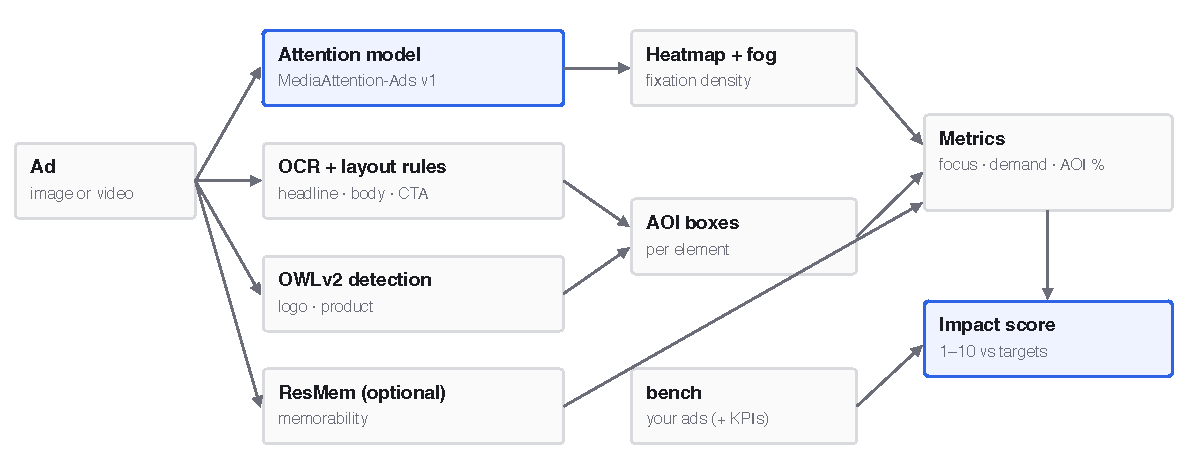
\includegraphics[width=\linewidth]{figs/pipeline.pdf}
\caption{The MediaAttention pipeline for one image. Video runs the same steps per frame, adds cut detection and tracks
areas of interest (AOIs) through each shot.}
\label{fig:pipeline}
\end{figure}

\subsection{Attention network}
We build on UNISAL~\cite{droste2020unisal} (Figure~\ref{fig:model}). A MobileNetV2~\cite{sandler2018mobilenetv2}
encoder (2.2M parameters) extracts features at 1/8, 1/16 and 1/32 scale. Sixteen learned Gaussian prior maps are
concatenated to the deepest features, letting the network learn content-independent viewing biases. A decoder with
skip connections upsamples the result; a domain-specific head applies a $1\times1$ adaptation, resizes to the input
and applies a learned $41\times41$ smoothing; a log-softmax produces a probability map over pixels. For video, a
convolutional GRU on a bypass between encoder and decoder carries state across frames; images skip it. Batch
normalisation, priors, adaptation and smoothing have one copy per data domain. We chose UNISAL as the base because it
is the most accurate model with a permissive licence in our webpage benchmark and is 17--70$\times$ faster than DeepGaze,
small enough to fine-tune on a laptop.

\begin{figure}[t]
\centering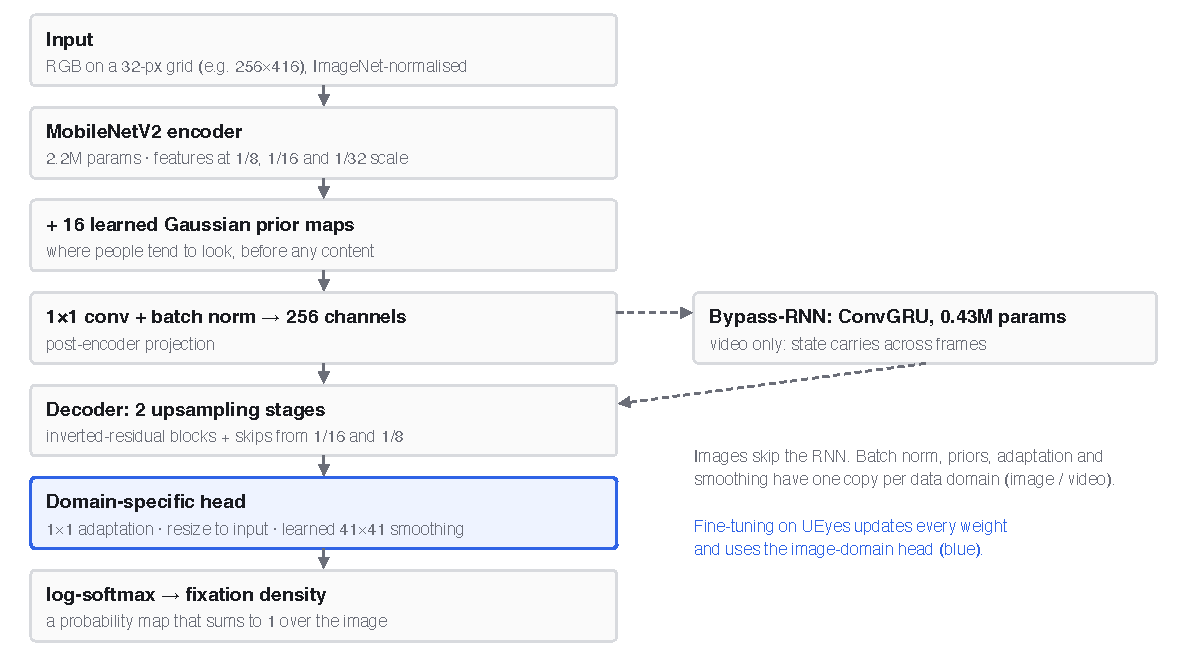
\includegraphics[width=0.92\linewidth]{figs/model.pdf}
\caption{The attention network (UNISAL architecture), 3.7M parameters in total.}
\label{fig:model}
\end{figure}

\subsection{Fine-tuning on design eye tracking}\label{sec:training}
\paragraph{Data.} We use the UEyes training split: 1,872 images (posters, mobile and desktop interfaces, webpages) with
eye tracking from 62 participants viewing freely for up to 7\,s on a Gazepoint GP3. A random 10\% (187 images) is held
out to select the epoch. The UEyes test split (108 images, 27 per category) and FiWI are never used for training or
model selection.

\paragraph{Targets.} Fixations inside each image are placed on a map and blurred with a Gaussian of about one degree of
visual angle (the dataset's 40 screen pixels per degree, converted to image pixels for each image's letterboxed
display). The map is resized to a quarter of the network input resolution and normalised to sum to one.

\paragraph{Loss and optimisation.} For predicted distribution $P$ and target $Q$ we minimise
\begin{equation}
\mathcal{L}(P,Q) = \mathrm{KL}(Q \,\|\, P) - \mathrm{CC}(P,Q),
\end{equation}
the usual pairing for saliency training: KL divergence penalises missed attention, correlation rewards the overall
shape. We start from UNISAL's SALICON weights and train all weights with AdamW (learning rate $3\times10^{-5}$, weight
decay $10^{-4}$), batch size one with batch-normalisation statistics frozen, for eight epochs (about 25 minutes on an
Apple M3 Pro). The epoch with the best held-out CC is kept. Nearly all of the gain arrives in the first epoch and the
curve then plateaus (Figure~\ref{fig:curve}), which suggests more data, rather than more training, is the next lever.
Only the image branch is tuned; video keeps UNISAL's DHF1K~\cite{wang2018dhf1k} weights, since no open ad-video
eye-tracking dataset exists.

\begin{figure}[t]
\centering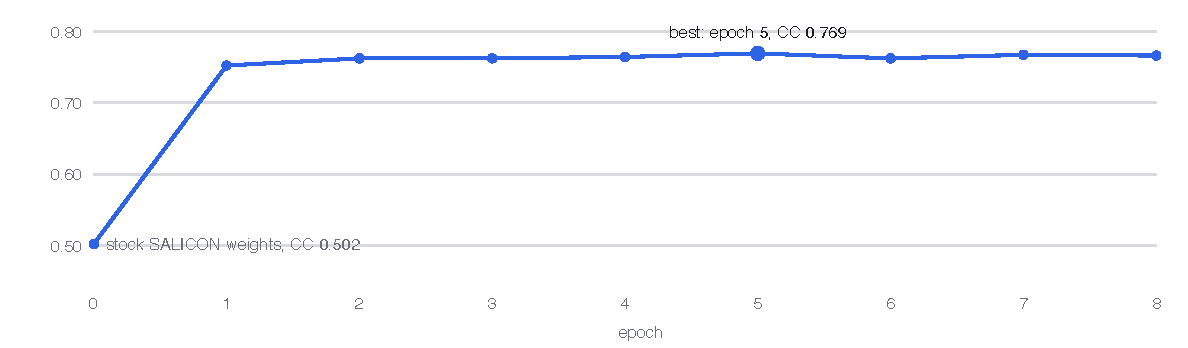
\includegraphics[width=0.85\linewidth]{figs/curve.pdf}
\caption{Held-out CC during fine-tuning (187 held-out training images). Epoch 0 is UNISAL's stock SALICON weights.}
\label{fig:curve}
\end{figure}

\subsection{From attention maps to advertising metrics}
Let $p$ be the predicted map normalised to sum to one over $N$ pixels.
\begin{itemize}
\item \textbf{Focus} (0--100). With pixels sorted by decreasing $p$, let $k$ be the smallest count whose mass reaches
0.8. Focus is $100\cdot\max(0,\, 1 - (k/N)/0.8)$: attention concentrated on a few elements scores high, evenly spread
attention scores zero.
\item \textbf{Cognitive demand} (0--100). The grayscale image is quantised to 32 levels and split into $16\times16$
blocks; the mean Shannon entropy~\cite{shannon1948} of the blocks is divided by $\log_2 32$, a simple clutter
measure~\cite{rosenholtz2007clutter}.
\item \textbf{Areas of interest.} OCR (PP-OCR~\cite{du2020ppocr}) reads every text line. Lines within 75\% of the
largest text height form the headline; a short line (at most four words) on a uniform patch covering at most 10\% of
the ad is the call to action, and its box grows to the button's edges; the remaining text is body copy.
OWLv2~\cite{minderer2023owlv2} detects the logo and the product. AOI attention is $\sum_{x\in\text{box}} p(x)$; lift is
attention share divided by area share.
\item \textbf{Memory} (optional). ResMem~\cite{needell2022resmem}, trained on LaMem~\cite{khosla2015lamem} and
MemCat~\cite{goetschalckx2019memcat}, predicts recognition after a brief exposure~\cite{isola2011memorable}.
\item \textbf{Impact Score} (1--10). Each metric scores 10 inside its target range and falls linearly from 7 at the
range edge to 1 at the end of the scale; the Impact Score is the mean. Targets are set from a folder of the user's own
ads: the top 20\% for higher-is-better metrics and the middle 50\% for cognitive demand, or, given campaign KPIs, the
middle 50\% of what the best-performing fifth of ads scored.
\item \textbf{Video.} A hard cut is a change of more than 40\% in the grayscale histogram, at least 0.5\,s after the
previous cut; messages placed right after cuts are easily forgotten~\cite{radvansky2011doorways}. AOIs found at the
start of each shot are tracked with pyramidal Lucas--Kanade optical flow~\cite{lucas1981iterative,shi1994good}, and
attention comes from the recurrent model fed at about six frames per second. Brand exposure over time follows
\cite{teixeira2010branding}.
\end{itemize}

\subsection{An open study kit}
Commercial tools rest on private panels. MediaAttention ships a static browser study instead: gaze is estimated from
webcam face landmarks with a per-participant ridge calibration on a 9-point grid followed by an accuracy check;
fixations are detected with a dispersion threshold; timed Yes/No word tests yield implicit scores weighted by each
participant's relative response speed; and a recognition test against foil ads measures memory. Nothing is uploaded:
participants download their own results file and choose whether to send it back. Webcam gaze is coarse (2--4 degrees
versus about 0.5 for lab trackers) but, aggregated over participants, suffices to validate heatmaps on one's own
creatives and is a route to openly licensed ad eye-tracking data.

\section{Benchmark}\label{sec:results}
\subsection{Setup}
\paragraph{Data.} FiWI~\cite{shen2014webpage}: 149 webpages at $1360\times768$, 11 viewers, 5\,s free viewing, ground
truth blurred with the dataset's own Gaussian ($\sigma=32$\,px). UEyes~\cite{jiang2023ueyes}: 1,980 images in four
categories; fixations are mapped to image pixels as in the dataset's own code and blurred with about one degree.
\paragraph{Models.} DeepGaze IIE and DeepGaze MSDB with a Gaussian centre-bias prior (MSDB with averaged dataset
parameters); TranSalNet-Dense with SALICON weights; UNISAL with SALICON weights; a Gaussian centre prior; and spectral
residual~\cite{hou2007spectral}. All are run as released, without fine-tuning, except MediaAttention-Ads v1.
\paragraph{Metrics and hardware.} pysaliency~\cite{kummerer2018benchmarking} computes AUC, sAUC, NSS, CC, SIM and KLD
per image; we average over images and report 95\% confidence intervals as $\pm1.96$ standard errors. Timing is on an
Apple M3 Pro (PyTorch MPS) after model loading. The full-UEyes DeepGaze MSDB run used a Colab T4 GPU with the same code.

\subsection{Webpages (FiWI)}
DeepGaze MSDB leads on every metric (Table~\ref{tab:fiwi}, Figure~\ref{fig:fiwi}). Every model is weakest on text-heavy
pages: stock UNISAL scores 0.531 on text pages against 0.676 on pictorial ones. Fine-tuning on design content raises
UNISAL's text-page CC to 0.597, the best of all models, and its overall CC from 0.616 to 0.631, although FiWI is out of
domain for both.

\begin{table}[t]
\centering\small
\resizebox{\linewidth}{!}{\begin{tabular}{lrrrrrrrr}
\toprule
Model & CC $\uparrow$ & NSS $\uparrow$ & sAUC $\uparrow$ & SIM $\uparrow$ & KLD $\downarrow$ & pictorial CC & mixed CC & text CC \\
\midrule
DeepGaze MSDB & 0.676 & 1.54 & 0.748 & 0.642 & 0.462 & 0.751 & 0.686 & 0.592 \\
DeepGaze IIE & 0.649 & 1.50 & 0.729 & 0.629 & 0.504 & 0.726 & 0.680 & 0.541 \\
\textbf{MediaAttention-Ads v1 (ours)} & \textbf{0.631} & \textbf{1.27} & \textbf{0.685} & \textbf{0.617} & \textbf{0.500} & \textbf{0.653} & \textbf{0.643} & \textbf{0.597} \\
UNISAL (stock) & 0.616 & 1.31 & 0.661 & 0.613 & 0.575 & 0.676 & 0.641 & 0.531 \\
TranSalNet-Dense & 0.608 & 1.25 & 0.646 & 0.605 & 0.603 & 0.650 & 0.642 & 0.532 \\
Centre-bias baseline & 0.345 & 0.62 & 0.500 & 0.476 & 0.899 & 0.305 & 0.373 & 0.358 \\
Spectral residual & 0.209 & 0.40 & 0.562 & 0.449 & 1.052 & 0.220 & 0.249 & 0.159 \\
\bottomrule
\end{tabular}
}
\caption{FiWI, 149 webpages; mean per-image scores, CC by page type on the right. No model was trained on FiWI.}
\label{tab:fiwi}
\end{table}

\begin{figure}[t]
\centering
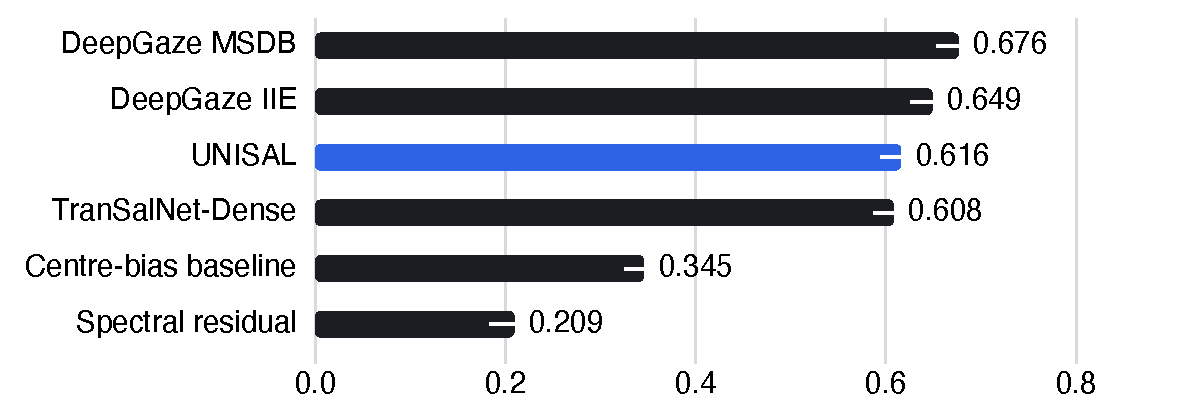
\includegraphics[width=0.49\linewidth]{figs/fiwi_bars.pdf}\hfill
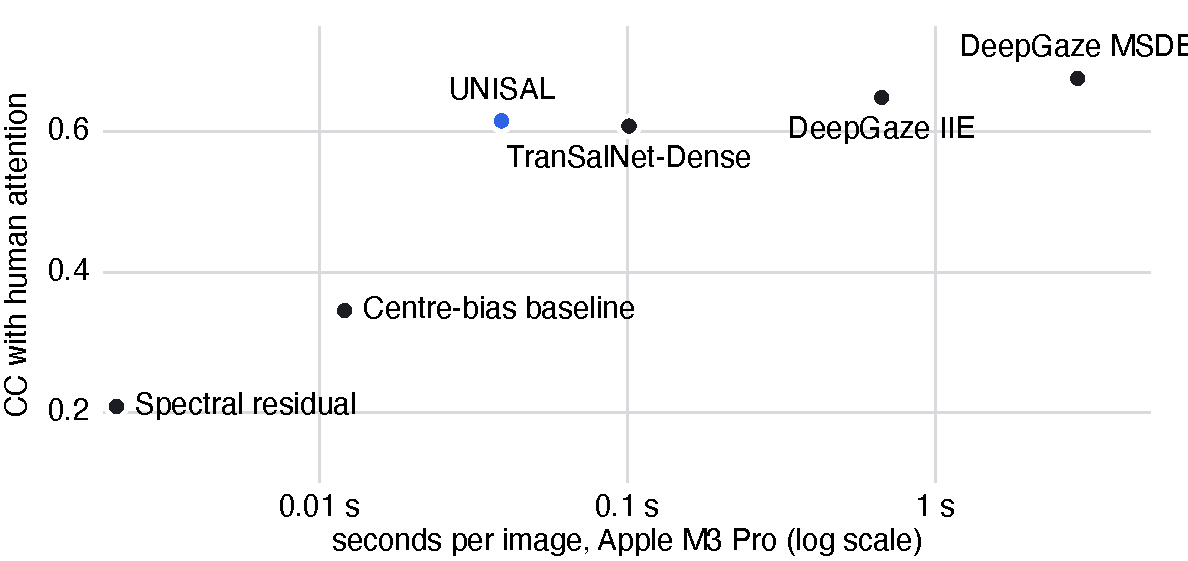
\includegraphics[width=0.49\linewidth]{figs/fiwi_speed.pdf}
\caption{FiWI. Left: CC with 95\% confidence intervals. Right: accuracy against inference time per image.}
\label{fig:fiwi}
\end{figure}

\subsection{Posters and interfaces (UEyes)}
Table~\ref{tab:ueyesfull} runs the released models on all 1,980 UEyes images. Every model is far weaker than on
webpages, and size does not help: the 452M-parameter DeepGaze MSDB ties the 104M-parameter DeepGaze IIE (CC 0.485) and
trails both TranSalNet (0.534) and the 3.7M-parameter UNISAL (0.502). MSDB does lead on sAUC, which removes centre
bias, so its ranking of salient regions is competitive; it is the shape of its maps that fits designed content poorly.

\begin{table}[t]
\centering\small
\resizebox{\linewidth}{!}{\begin{tabular}{lrrrrrrrrr}
\toprule
Model & CC $\uparrow$ & NSS $\uparrow$ & sAUC $\uparrow$ & SIM $\uparrow$ & KLD $\downarrow$ & poster CC & mobile CC & desktop CC & web CC \\
\midrule
TranSalNet-Dense & 0.534 & 1.01 & 0.655 & 0.586 & 0.700 & 0.523 & 0.586 & 0.543 & 0.483 \\
UNISAL (stock) & 0.502 & 0.97 & 0.656 & 0.573 & 0.779 & 0.494 & 0.521 & 0.526 & 0.468 \\
DeepGaze MSDB & 0.485 & 0.99 & 0.704 & 0.525 & 0.921 & 0.463 & 0.516 & 0.517 & 0.443 \\
DeepGaze IIE & 0.485 & 0.95 & 0.684 & 0.548 & 0.777 & 0.483 & 0.478 & 0.513 & 0.465 \\
Spectral residual & 0.232 & 0.45 & 0.623 & 0.463 & 1.006 & 0.257 & 0.198 & 0.290 & 0.185 \\
Centre-bias baseline & 0.220 & 0.37 & 0.497 & 0.468 & 0.963 & 0.257 & 0.201 & 0.198 & 0.225 \\
\bottomrule
\end{tabular}
}
\caption{All 1,980 UEyes images, models as released. MediaAttention-Ads v1 is excluded because it was trained on the
training split; see Tables~\ref{tab:ueyestest} and~\ref{tab:posters}.}
\label{tab:ueyesfull}
\end{table}

On the held-out test split (Table~\ref{tab:ueyestest}), MediaAttention-Ads v1 reaches CC 0.735 against 0.514 for the
best other model, and leads in every category by 0.19 to 0.26. On posters, the category closest to print and display
advertising, it reaches 0.752 [0.695, 0.809] against 0.496 [0.440, 0.551] for TranSalNet (Table~\ref{tab:posters});
the intervals do not overlap.

\begin{table}[t]
\centering\small
\resizebox{\linewidth}{!}{\begin{tabular}{lrrrrrrrrr}
\toprule
Model & CC $\uparrow$ & NSS $\uparrow$ & sAUC $\uparrow$ & SIM $\uparrow$ & KLD $\downarrow$ & poster CC & mobile CC & desktop CC & web CC \\
\midrule
\textbf{MediaAttention-Ads v1 (ours)} & \textbf{0.735} & \textbf{1.53} & \textbf{0.731} & \textbf{0.680} & \textbf{0.399} & \textbf{0.752} & \textbf{0.820} & \textbf{0.692} & \textbf{0.674} \\
TranSalNet-Dense & 0.514 & 1.00 & 0.646 & 0.559 & 0.771 & 0.496 & 0.601 & 0.482 & 0.476 \\
UNISAL (stock) & 0.467 & 0.92 & 0.640 & 0.543 & 0.864 & 0.454 & 0.504 & 0.456 & 0.452 \\
DeepGaze IIE & 0.454 & 0.92 & 0.667 & 0.522 & 0.871 & 0.458 & 0.460 & 0.453 & 0.445 \\
DeepGaze MSDB & 0.452 & 0.94 & 0.690 & 0.499 & 1.039 & 0.415 & 0.530 & 0.465 & 0.397 \\
Centre-bias baseline & 0.219 & 0.40 & 0.499 & 0.447 & 1.021 & 0.281 & 0.189 & 0.190 & 0.215 \\
Spectral residual & 0.214 & 0.44 & 0.616 & 0.433 & 1.125 & 0.285 & 0.131 & 0.270 & 0.169 \\
\bottomrule
\end{tabular}
}
\caption{UEyes test split, 108 images (27 per category) never used for training or model selection.}
\label{tab:ueyestest}
\end{table}

\begin{table}[t]
\centering\small
\begin{tabular}{lrcrr}
\toprule
Model & CC $\uparrow$ & 95\% CI & NSS $\uparrow$ & KLD $\downarrow$ \\
\midrule
\textbf{MediaAttention-Ads v1 (ours)} & \textbf{0.752} & \textbf{[0.695, 0.809]} & \textbf{1.55} & \textbf{0.354} \\
TranSalNet-Dense & 0.496 & [0.440, 0.551] & 0.98 & 0.792 \\
DeepGaze IIE & 0.458 & [0.392, 0.524] & 0.90 & 0.894 \\
UNISAL (stock) & 0.454 & [0.389, 0.518] & 0.90 & 0.913 \\
DeepGaze MSDB & 0.416 & [0.351, 0.481] & 0.86 & 1.079 \\
Spectral residual & 0.285 & [0.209, 0.361] & 0.58 & 1.082 \\
Centre-bias baseline & 0.281 & [0.218, 0.344] & 0.55 & 0.949 \\
\bottomrule
\end{tabular}

\caption{UEyes test posters ($n=27$), with 95\% confidence intervals over images.}
\label{tab:posters}
\end{table}

\begin{figure}[t]
\centering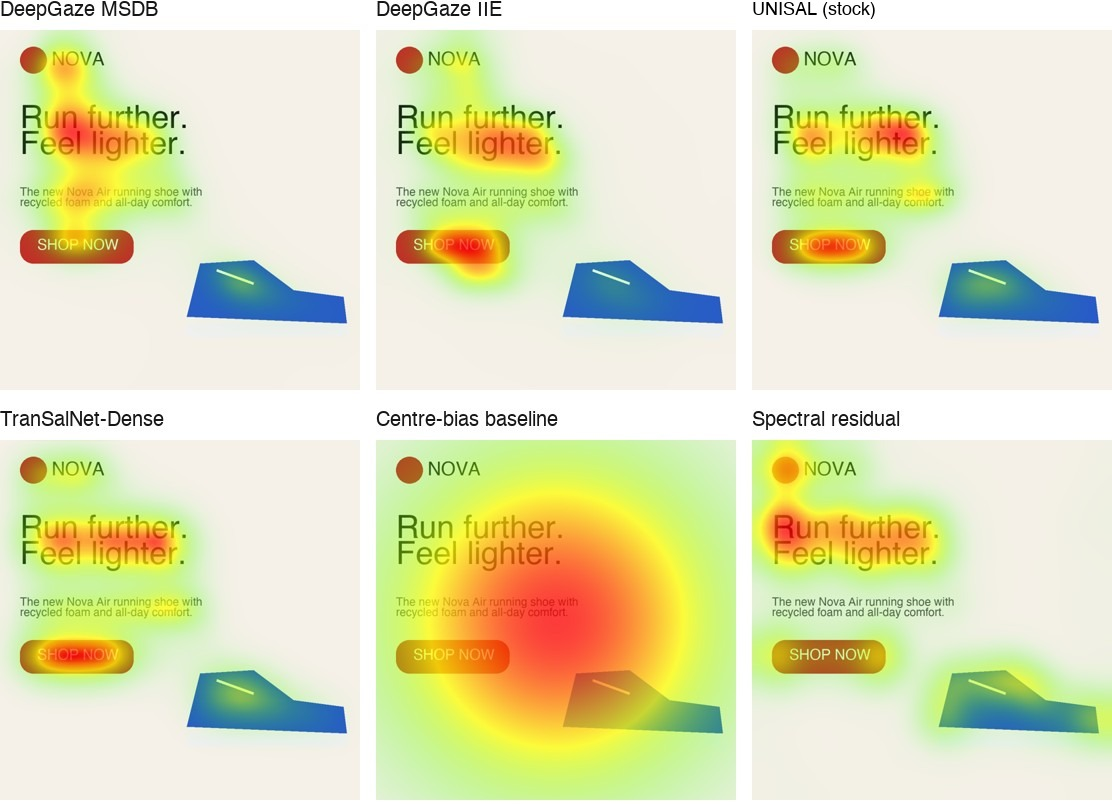
\includegraphics[width=\linewidth]{figs/models_on_ad.jpg}
\caption{Predictions of the benchmarked models on the same synthetic ad (illustrative; no ground truth).}
\label{fig:qual}
\end{figure}

\subsection{Architectures compared}
Table~\ref{tab:arch} sets the models side by side: UNISAL (Figure~\ref{fig:model}); TranSalNet, a DenseNet-161 CNN with a transformer encoder and CNN decoder; DeepGaze IIE, an ensemble of four ImageNet backbones with a readout network; DeepGaze MSDB, CLIP RN50x64 and DINOv2 ViT-B/14 features at several scales with dataset-bias parameters; and, for reference, the commercial Neurons model, a CNN encoder--decoder with ConvNeXt and ResNet-50 components trained on proprietary eye tracking from about 20,000 participants~\cite{neurons2025tech}. MediaAttention-Ads v1 is 20--120$\times$ smaller and 17--70$\times$
faster than the DeepGaze models, handles images and video in one network, and is the only accurate model whose code
and weights carry a permissive licence; the DeepGaze repositories have no licence file. Its weakness is photo-led
content: DeepGaze MSDB remains about 0.05 CC ahead on FiWI and further ahead on pictorial pages.

\begin{table}[t]
\centering\small
\resizebox{\linewidth}{!}{\begin{tabular}{lrllrrr}
\toprule
Model & Params & Video & Licence & s / image & UEyes test CC & FiWI CC \\
\midrule
\textbf{MediaAttention-Ads v1 (ours)} & \textbf{3.7M} & \textbf{yes (recurrent)} & \textbf{Apache-2.0} & \textbf{0.04} & \textbf{0.735} & \textbf{0.631} \\
UNISAL (stock) & 3.7M & yes (recurrent) & Apache-2.0 & 0.04 & 0.467 & 0.616 \\
TranSalNet-Dense & 76.6M & no & MIT & 0.10 & 0.514 & 0.608 \\
DeepGaze IIE & 104.0M & no & none & 0.67 & 0.454 & 0.649 \\
DeepGaze MSDB & 451.6M & no & none & 2.90 & 0.452 & 0.676 \\
Neurons (commercial) & n/d & separate model & closed & -- & n/a & n/a \\
\bottomrule
\end{tabular}
}
\caption{Size, video support, licence, speed (Apple M3 Pro) and accuracy (CC). Parameter
counts were measured by loading each model. The commercial model is described from its public tech
paper~\cite{neurons2025tech} and could not be run.}
\label{tab:arch}
\end{table}

\section{Discussion and limitations}
\paragraph{What predicted attention can tell an advertiser.} Models trained on free viewing predict bottom-up attention
in the first seconds: what pops out. They do not model goal-directed search, audio, or the placement context of an ad.
Predicted attention is a fast first filter for comparing creative variants, not a replacement for testing with people
when stakes are high. Buyers should ask vendors for CC and NSS on held-out, third-party-scored data rather than a bare
percentage.

\paragraph{Limitations.} FiWI is small (149 pages, 11 viewers). UEyes is one lab panel of 62 participants viewing freely
for up to 7\,s; neither measures a one-second glance in a scrolling feed, and cultural coverage is narrow. Our model's
video branch is not ad-tuned or validated on ad eye tracking, and the secondary metrics (focus, cognitive demand,
memory) have not been validated against campaign outcomes. Commercial tools could not be run on the same data.

\paragraph{Future work.} Tuning the recurrent branch on ad video, scoring creatives in feed context with short
exposures, distilling a larger model on photographs while keeping the design data, and growing an open ad
eye-tracking dataset with the study kit.

\section{Conclusion}
Commercial attention-prediction claims are rarely comparable, and where third-party scores exist, the best open models
match or beat them. On designed content, larger models do not help; training on design eye tracking does. A
3.7M-parameter network fine-tuned on UEyes for 25 minutes on a laptop leads every open model on posters, ads and
interfaces by more than 0.2 CC and runs in tens of milliseconds. The model, toolkit, benchmark and study kit are open.

\paragraph{Availability.} Code (Apache-2.0), benchmark scripts, per-image results and the study kit:
\url{https://github.com/pranikz/MediaAttention}~\cite{mahapatra2026mediaattention}. Model weights (Apache-2.0):
\url{https://huggingface.co/pranikz/MediaAttention-Ads}. MediaAttention-Ads v1 is a fine-tune of UNISAL (Apache-2.0)
on UEyes (CC BY 4.0); no UEyes images are redistributed.

\bibliographystyle{unsrtnat}
\bibliography{refs}
\end{document}
